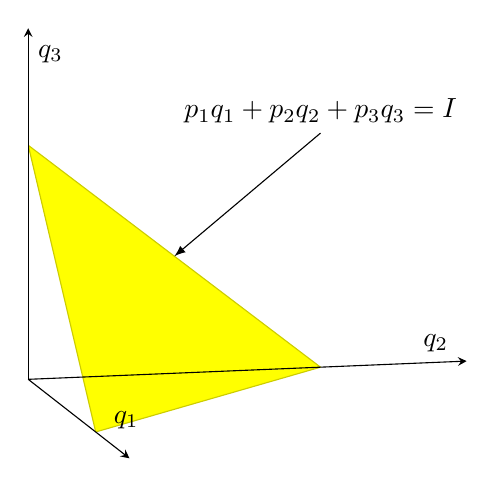
\begin{tikzpicture}
  \begin{axis}[view={77}{13},
      axis lines=middle,
      axis on top,
      ticks=none,
      clip=true,
      patch,
      xlabel={$q_1$},
      ylabel={$q_2$},
      zlabel={$q_3$},
      samples=50,
      xmin=0,
      xmax=1.5,
      ymin=0,
      ymax=1.5,
      zmin=0,
      zmax=1.5,
      domain=0:1,
      domain y=0:1,]
    \addplot3[surf] coordinates {
      (1,0,0) 
      (0,1,0) 
      (0,0,1)
    };
    \node[anchor=south] at (0, 1, 1) {$p_1q_1 + p_2 q_2 + p_3q_3 = I$};
    \draw[-latex] (0, 1, 1) -- (0, 0.5, 0.5) ;
  \end{axis}
\end{tikzpicture}

